\par\addvspace{12pt}\Needspace{9\baselineskip}

\section{数据的描述}

% ITEM: probability-example-028
\solutionitem{probability-example-028}{例6.28}
甲组20个数据，均值为60、方差为4；乙组30个数据，均值为70、方差为9。求合并后的均值与描述方差，再讨论两组均值相同时公式怎样简化。
\solutionanswer
合并均值\(0.4\times60+0.6\times70=66\)。组内方差平均\(0.4\times4+0.6\times9=7\)，组间贡献\(0.4(60-66)^2+0.6(70-66)^2=24\)，故描述方差\(31\)。若两组均值相同，组间项为零，合并方差就是组内方差按人数加权的平均。


% ITEM: probability-example-029
\solutionitem{probability-example-029}{例6.29}
（据2025年上海卷改编）
历届奥运会男子\(4\times100\)米混合泳接力冠军的十个成绩数据如下，单位为秒，已按升序排列：
\[
\begin{array}{rrrrr}
206.78&207.46&207.95&209.34&209.35\\
210.68&213.73&214.84&216.93&216.93
\end{array}
\]
求极差、中位数与样本均值；从这十条记录中随机选三条，求恰有两条成绩大于211秒的概率。
\solutionanswer
极差\(216.93-206.78=10.15\)秒，中位数\((209.35+210.68)/2=210.015\)秒，样本均值\(211.399\)秒。大于211秒的记录有4条，其余6条，所以所求概率\(\binom42\binom61/\binom{10}3=3/10\)。两个相同的216.93仍是两条不同记录。


% ITEM: probability-exercise-19-01
\solutionitem{probability-exercise-19-01}{习题6.19（1）}
对数据\(2,3,3,4,5,7,7,9\)，求均值、中位数、众数、四分位距与描述方差，并画箱线图。
\solutionanswer
均值为\(5\)，中位数\((4+5)/2=4.5\)，众数\(3,7\)。按本书约定\(Q_1=(3+3)/2=3,Q_3=(7+7)/2=7\)，四分位距\(4\)。描述方差为\([4+9+9+16+25+49+49+81]/8-25=21/4\)。箱体从3到7，中位线为4.5，两须到2和9，如图。
\begin{center}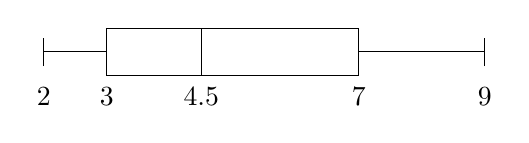
\begin{tikzpicture}[x=.8cm,y=.6cm]
\draw(2,0)--(3,0);\draw(7,0)--(9,0);\draw(2,-.3)--(2,.3);\draw(9,-.3)--(9,.3);\draw(3,-.5)rectangle(7,.5);\draw(4.5,-.5)--(4.5,.5);
\foreach \x/\a in {2/2,3/3,4.5/4.5,7/7,9/9}{\node[below]at(\x,-.55){$\a$};}
\end{tikzpicture}\end{center}


% ITEM: probability-exercise-19-02
\solutionitem{probability-exercise-19-02}{习题6.19（2）}
正文所指右图如下，柱高为频率除以组距。
\begin{center}\includegraphics[width=.74\linewidth]{probability-histogram-exam}\end{center}
（据2020年天津卷第4题改编）由图6.6右图，求80个零件中直径在\([5.43,5.47)\)毫米内的个数，并估计该批产品中此类零件的比例。
\solutionanswer
对应两根柱的高度为\(6.25,5\)，组距均为\(0.02\)。频率是矩形面积之和，\(0.02(6.25+5)=0.225\)，故80件中有\(80\times0.225=18\)件；以此估计该批比例为\(22.5\%\)。


% ITEM: probability-exercise-19-03
\solutionitem{probability-exercise-19-03}{习题6.19（3）}
两组人数相等，均值为\(\mu\pm d\)，方差均为\(v\)。求合并后的均值与方差。
\solutionanswer
合并均值为\(\mu\)。两组权重各\(1/2\)，组内平均方差\(v\)，组均值偏差平方都为\(d^2\)，所以合并方差\(v+d^2\)。


% ITEM: probability-exercise-19-04
\solutionitem{probability-exercise-19-04}{习题6.19（4）}
分别构造均值相同而方差不同，以及均值方差相同而形态不同的两组数据。
\solutionanswer
例如\((0,0)\)和\((-1,1)\)均值都是零，方差分别为零、1。再取\((-1,-1,1,1)\)与\((-\sqrt2,0,0,\sqrt2)\)，均值均零、描述方差均1，前一组分在两侧，后一组有一半集中在中心，形态不同。均值和方差并未完整记录分布。
\par
